\chapter{Mitigation Strategies}
\label{chap:mitigationstrats}

\section{Nature-based Solutions for bank erosion}

When it comes to Nature-based solutions, the question arises what this definition means. A quite general definition of nature based solutions would be;

\textit{“Nature-based Solutions are actions to protect, conserve, restore, sustainably
use and manage natural or modified terrestrial, freshwater, coastal and marine
ecosystems, which address social, economic and environmental challenges
effectively and adaptively, while simultaneously providing human well-being,
ecosystem services, resilience and biodiversity benefits” (United Nations, 2022,
p. 2)}

Although this definition may give a thought that it only concerns natural and biodiversity increasing ideas this is actually not the case. For example the impact of NBS on the local economies and communities is of an equal importance. When it comes to weighing the different NBS against each other this report will make use of the seven goals of the IUCN which must be achieved as good as possible. The seven goals are presented below;

\begin{figure}[H]
    \centering
    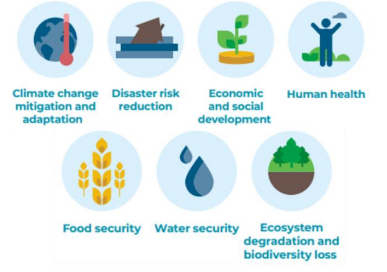
\includegraphics[width=0.50\linewidth]{figures/ThesevenNBSgoals.png}
    \caption{Seven goals for achieving a good NBS}
    \label{fig:placeholder}
\end{figure}

\subsection{Resistance against NBS}

Although NBS are widely known in the scientific world, most people have never heard of these solutions. So, when implementing a solution which can't be described as a classical solution, there is a big change of getting resistance from multiple stakeholders. Especially local communities are skeptical because the solution is less concrete than a classical solution would be. The business case of a NBS must of course also be solid. Without funding of the project, there will never be a change to realize it. That's why it's from great importance to have a solution which is both profitable as explainable to the stakeholders. 

\subsection{Implementing NBS in this project}

As stressed out before in this report, is there a problem with riverbank erosion due to activities on the river. To mitigate or even solve this problem, it is our intend to use a nature based solution. Therefore there are presented multiple possible solutions to create a long-lasting, sustainable riverbank which is made cost effective. These solutions are all graded from one to ten for the seven goals described in section 7.1. The solution which has the highest score will be chosen to mitigate the bank erosion.

One of these solutions is to make a, so said, buffer zone. This means that there is made a swamp area of about 2-8 meter. This gives a change for plants which will hold the soil together. By holding the soil together there will in time be a muddy and organic soil composition, which gives a lot of room for plants and animals to flourish. By doing so, there won't be any erosion on the banks of the river. 


\subsection{Bed and bank protection measures}

belangrijke/interessante info over deltas en wetlands:
The Paraná Delta, the end of the Paraná-Paraguay river wetland system, begins in the city of Diamante in Entre Ríos province. It stretches for 300 kilometres and covers some 2.3 million hectares. Dotted with islands, these wetlands are a source of ecosystem services such as flood and drought buffering, water purification, erosion control and coastal protection, climate regulation, as well as the provision of shelter, feeding and breeding sites for various wildlife species. It also provides resources including fish, foraging, timber, medicine, and materials for construction and clothing.

In recent years, wetlands have become increasingly important for another key reason: their role as allies against climate change. They improve the resilience of communities to its impacts, serve as natural barriers against floods and droughts, and also function as carbon sinks. Despite playing these important roles, these ecosystems remain under great threat from human action – it is estimated that globally, 85 percent of the wetlands that existed three centuries ago have been destroyed or drastically transformed. 

https://dialogue.earth/en/climate/on-the-parana-river-ecological-crisis-is-a-threat-to-its-identity/


\newpage

\section{Structural Solutions for Bank Erosion}
\label{section_8.2}

There are a number of retaining structures that can be used to stabilize the river banks. Possibilities include:
\begin{itemize}
    \item Sheet pile wall\\
    Sheet pile walls are a common retaining structure and consist of vertical barriers made of interlocking sections. They are a lightweight option and can be removed, which makes them reusable across multiple projects. Another advantage is the fact that installation is relatively easy and therefore cheap. However, sheet pile walls also have limitations. In hard soils and soils with boulders or cobbles, installation becomes difficult. Further, installation can disturb nearby areas through sounds and vibrations. These vibrations can even cause settlements to occur \autocite{korffReaderDeepExcavations2023}.

    \item Diaphragm wall\\
    Diaphragm walls are deep, reinforced concrete retaining structures. They provide excellent structural stability and are capable of resisting significant lateral soil and water pressures. One of their key advantages is water tightness, as they effectively prevent groundwater seepage. They are also suitable for a wide range of soil conditions, and offer durability due to the use of reinforced concrete. On the downside, they are costly to build and require significant time and space due to the specialized equipment, skilled labor, and extensive excavation work that is needed \autocite{korffReaderDeepExcavations2023}.
    
    \item Precast concrete wall\\
    Precast concrete walls are constructed by manufacturing structural elements in a factory environment before transporting them to the construction site. This process allows for superior quality control. Moreover, precast construction can significantly speed up project timelines, as elements are produced in large quantities and quickly installed on-site. Precast concrete offers a long service life with minimal maintenance. Drawbacks of precast concrete walls include: the elements are heavy and thus require specialized transportation and installation equipment \autocite{mcneilengineeringAdvantagesDisadvantagesUsing2023}. Further, the production and transport processes have notable environmental impacts, and repairs or replacements can be complex and costly.

    \item Auger pile wall or soldier pile wall\\
    Auger pile walls and soldier pile walls are widely used in construction for retaining slopes. Auger pile walls are formed by drilling and casting concrete in place, while soldier pile walls consist of vertical steel or timber H-piles with horizontal boards or panels placed between them. They are generally cost-effective solutions that generate minimal vibrations, making them suitable for urban areas and sites sensitive to noise or disturbance. Both systems offer flexibility, allowing adjustments to pile placement, size, and depth to suit specific project requirements. However, leakage between adjacent piles is a relevant risk when it comes to these types of walls \autocite{korffReaderDeepExcavations2023}. Maintaining proper overlap between piles is also critical to ensure structural stability and continuity of the wall.
\end{itemize}

In Table \ref{tab:compstruct}, the different structural solutions are summarized and are scored on different relevant criteria.

\begin{table}[H]
\centering
\caption{Comparison of structural solutions}
\resizebox{\textwidth}{!}{%
\begin{tabular}{lcccccccc}
\hline
Method & Installation & Price & Resistance & Versatility & Disturbance & Water tightness & Durability & Sustainability \\
\hline
Sheet pile wall & ++ & + & + & - & - & 0 & + & ++ \\
Diaphragm wall  & -- & -- & ++ & ++ & + & ++ & ++ & - \\
Precast concrete wall & - & - & ++ & 0 & ++ & + & + & -- \\
Auger/Soldier pile wall & + & ++ & 0 & + & ++ & -- & - & 0 \\
\hline
\end{tabular}%
}
\label{tab:compstruct}
\end{table}

As can be seen in Table \ref{tab:compstruct}, pile walls score low on water tightness and durability. The area of interest is located in a delta and hence high groundwater levels are to be expected. Therefore, water tightness must be guaranteed. Since the pile walls don't offer this certainty, this option is not further discussed. The diaphragm wall, on the other hand, offers great water tightness but installation is a far bigger challenge for this method. The benefits that the diaphragm wall offers, great resistance and low disturbance being the most relevant ones, do not outweigh the cons: the large amounts of time, space and budget needed to construct them. The same is true for the precast concrete wall: the heavy elements ask for a specialized and expensive installation procedure. The specialized equipment and experience is possibly not available or expensive, which means the precast concrete walls are not a viable option.

As a structural solution, the sheet pile walls are chosen. These elements score high on ease of installation and sustainability (parts can be removed and reused) and price, resistance and durability are also pros of this method. Disturbance is one of the main concerns related to sheet pile walls, but since the area of interest is in a scarcely populated area, this is not necessarily problematic. Another concern is the low versatility: installation is only possible if soils are not too hard. However, since installation will be executed in a delta with relatively soft soil (see xx), this should not be a major concern for this project.

\subsection{Sheet Pile Wall}
\label{section:sheet_pile_wall}

Sheet pile walls are frequently used in practices for application like excavations, waterfront structures, highway structures, flood protections schemes and bridge abutments. Steel sheet pile walls are mostly used as the high variety of combinations and the various profiles achieve the high moments of resistance while still maintaining the structural requirements of the design. In addition, the engineering advantages are in line with their suitability for water use, favorable ratio of steel cross section and moment of resistance and fast progress on site, which including their functionality and economical benefits is making their use favorable (Handbook).

The types of steel sheet pile walls which are most used in practice are the cantilever walls and anchored walls. Cantilever walls are mostly used as flood walls or earth retaining walls with heights of 3 to 5 meters. They are getting their support reactions from the ground and foundation soils and can be seen in Figure \ref{fig:sheetpiles}. The anchored walls can be used when the heights of cantilever walls are exceeded or when the design should be based on lateral deflections. However, within this design the horizontal distance which will be required for the installation should be considered and and configuration can be seen in Figure \ref{fig:sheetpiles} (EM-1110).

\begin{figure}[H]
    \centering
    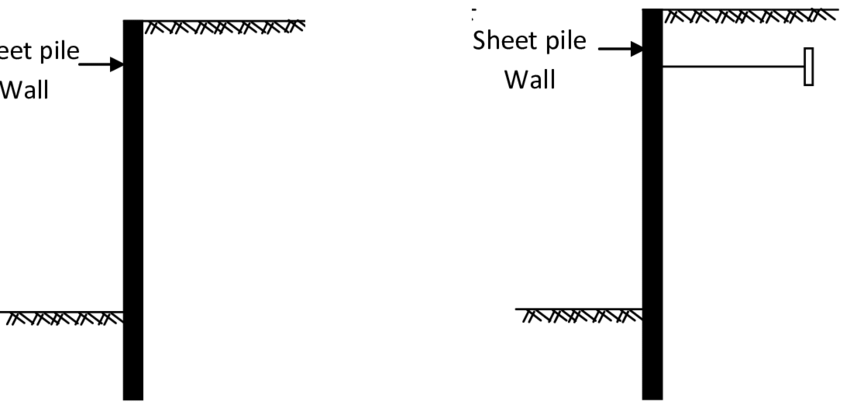
\includegraphics[width=0.50\linewidth]{figures/ch8/Anchored-Sheet-pile-wall.png}
    \caption{Cantilever and anchored sheet pile wall}
    \label{fig:sheetpiles}
\end{figure}

Sheet pile walls can be made of multiple materials, like steel, concrete, or wood. In this report, steel sheet pile walls will be used as advantages of this material outweighs the disadvantages and is more suitable than concrete or wood. As concrete will have a long service live, however, it will have high initial costs compared to steel and the installation of concrete walls is more difficult in relation to steel ones. In addition, wood walls, can only be used for short heights and will only be used for temporary structures. Like discussed in Section \ref{section_8.2} the advantages of steel piles and making it therefore the most common material used is the strength, light weight and long service life, in combination with the favorable ratio of cross-section and moment of resistance (EM-1110).

\subsubsection{Sections and interlocks}

For steel sheet pile walls, the sections and interlocks are of importance to make a complete wall which can be used for the application of waterfront structures. Figure \ref{fig:sections_sheetpiles} shows typical steel sections widely used and are known by the names of U and Z sections. In this figure the interlocks, which gives the sections its strength can also be seen. While the interlocks of the U sections are on the neutral axis, the ones for the Z sections are not. The maximum shear stress, can be obtained in the neutral axis, which makes the interlocks should be welded or crimped to obtain the full moment of resistance. When walls are in touch with water, and the walls need to be watertight, materials to fill up the interlocks like plastic compounds or the use of a preformed polyurethane interlock seal can be taken into considerations. 

\begin{figure}[H]
    \centering
    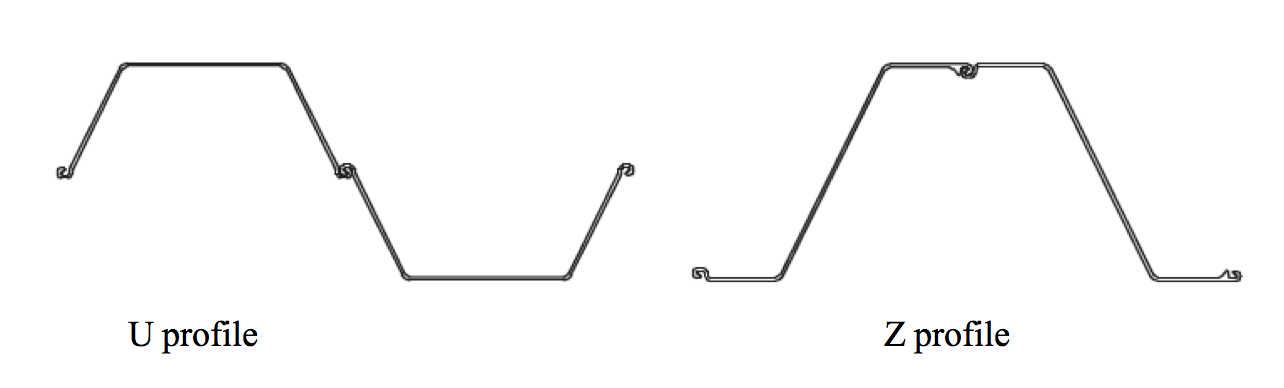
\includegraphics[width=0.50\linewidth]{figures/ch8/u_profile_z_profile.png}
    \caption{U and Z sections}
    \label{fig:sections_sheetpiles}
\end{figure}

\subsubsection{Properties of steel}

As steel will be the material used for the sheet piles the properties of steel, as being a homogeneous material will be touched on. Steel is an elastic material and has a favorable strength to weight ratio while characterizing the a range of 300 $N/mm^{2}$ to 2000 $N/mm^{2}$ for the tensile strength of this material. The stress-strain behavior of steel can be seen in Figure \ref{fig:stress_strain_steel}. The range of elasticity is depending on the grade of the steel and the elastic modulus for steel is 210000 $N/mm^{2}$. In Figure \ref{fig:stress_strain_steel}, $f_{y}$ is characterized as the yield strength which is the value where the stress will be constant or drop or go to a strain of 0.2\% when the load is taken away. Furthermore, $f_{u}$, is the tensile strength which is in line with the steel grade (Handbook).

\begin{figure}[H]
    \centering
    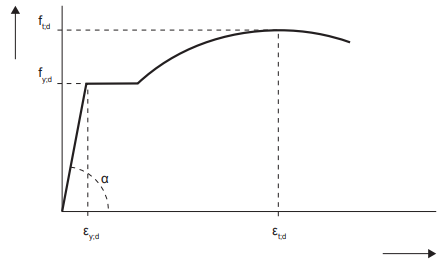
\includegraphics[width=0.50\linewidth]{figures/ch8/stress_strain_steel.png}
    \caption{Stress-strain relation steel}
    \label{fig:stress_strain_steel}
\end{figure}

The mechanical properties of steel grades which are used for sheet piles are shown in Table \ref{tab:steel_materialproperties}. Steel sheet piles are made of hot rolled sections, which is the process of heating the steel to temperatures of over 900 $^{\circ}$C, before rolling which allows for the various shape and sizes what is of importance with sheet piles. Hot rolled sections are having slightly rougher surface when comparing it to cold rolled sections (BuyABeam). 

\begin{table}[ht]
  \centering
  \caption{Mechanical properties by steel grade}
  \label{tab:steel-grades}
  \setlength{\tabcolsep}{10pt}
  \renewcommand{\arraystretch}{1.25}
  \begin{tabular}{lccc}
    \toprule
    \textbf{Steel grade}
    & \textbf{Tensile strength} $f_{u}\,[\mathrm{N/mm}^{2}]$
    & \textbf{Yield strength} $f_{y}\,[\mathrm{N/mm}^{2}]$
    & \textbf{Elongation at failure} $\varepsilon_{u}\,[\%]$ \\
    \midrule
    S 240 GP & 340 & 240 & 26 \\
    S 270 GP & 410 & 270 & 24 \\
    S 320 GP & 440 & 320 & 23 \\
    S 355 GP & 480 & 355 & 22 \\
    S 390 GP & 490 & 390 & 20 \\
    S 430 GP & 510 & 430 & 19 \\
    \bottomrule
    \label{tab:steel_materialproperties}
  \end{tabular}
\end{table}

\subsubsection{Failure mechanisms}

\begin{figure}[H]
    \centering
    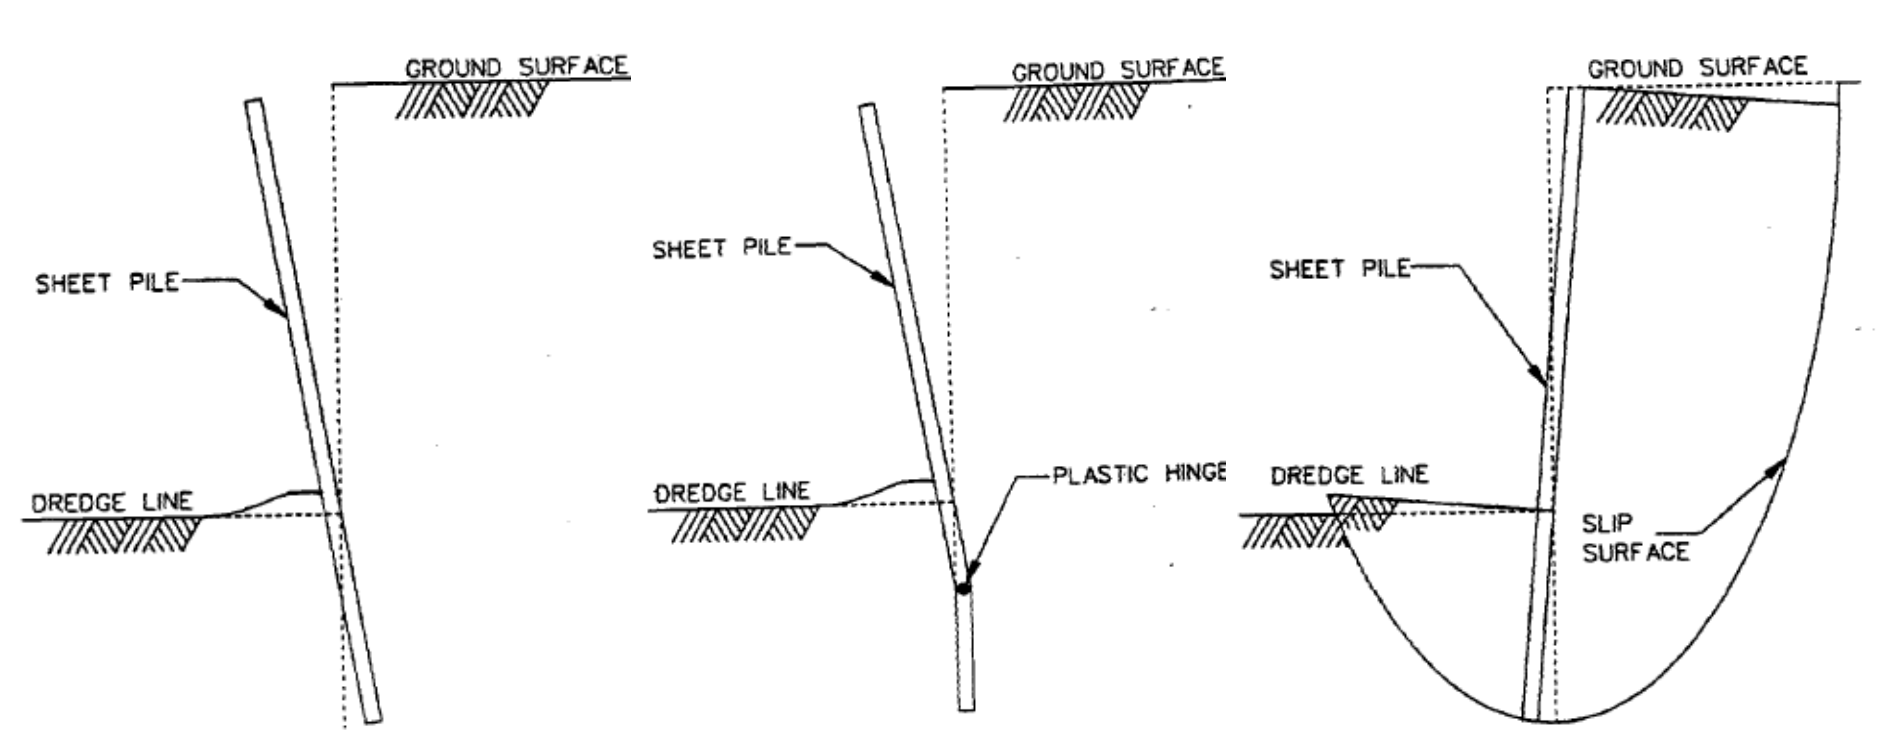
\includegraphics[width=0.70\linewidth]{figures/ch8/failure_mechanisms.png}
    \caption{Failure mechanisms cantilever sheet pile wall}
    \label{fig:failure_mechanisms_sheetpiles}
\end{figure}

\subsection{Design of heet pile wall}

To design the steel sheet pile wall, first the critical location and a problem description should be identified to get a better understanding of the situation. After defining the conditions, a method should be considered to calculate the earth pressure and water pressure to later balance the moments to iteratively define the depth of the sheet pile wall. The sheet pile wall with the retaining height and embedded depth will after be verified based on the structural verifications including bending moments, shear force, and deflection of the wall. The soil parameters are defined and the soil profile is taken from Section XX while the water levels are taken from Section XX. These will be further analyzed and used for the design of the sheet pile.

\subsubsection{Critical locations}

The determination of the critical erosion points along the river has been done in Section \ref{section:cirtical_location}. The location which is analyzed here will also be the critical location where the design of the steel sheet pile will be based on. In Figure \ref{fig:critical_location}, the critical point in shown in Aqua Monitor and during the field trip images have been made to verify if the critical location of the Aqua Monitor map was visible. 

\begin{figure}[H]
    \centering
    \begin{subfigure}[b]{0.45\textwidth}
        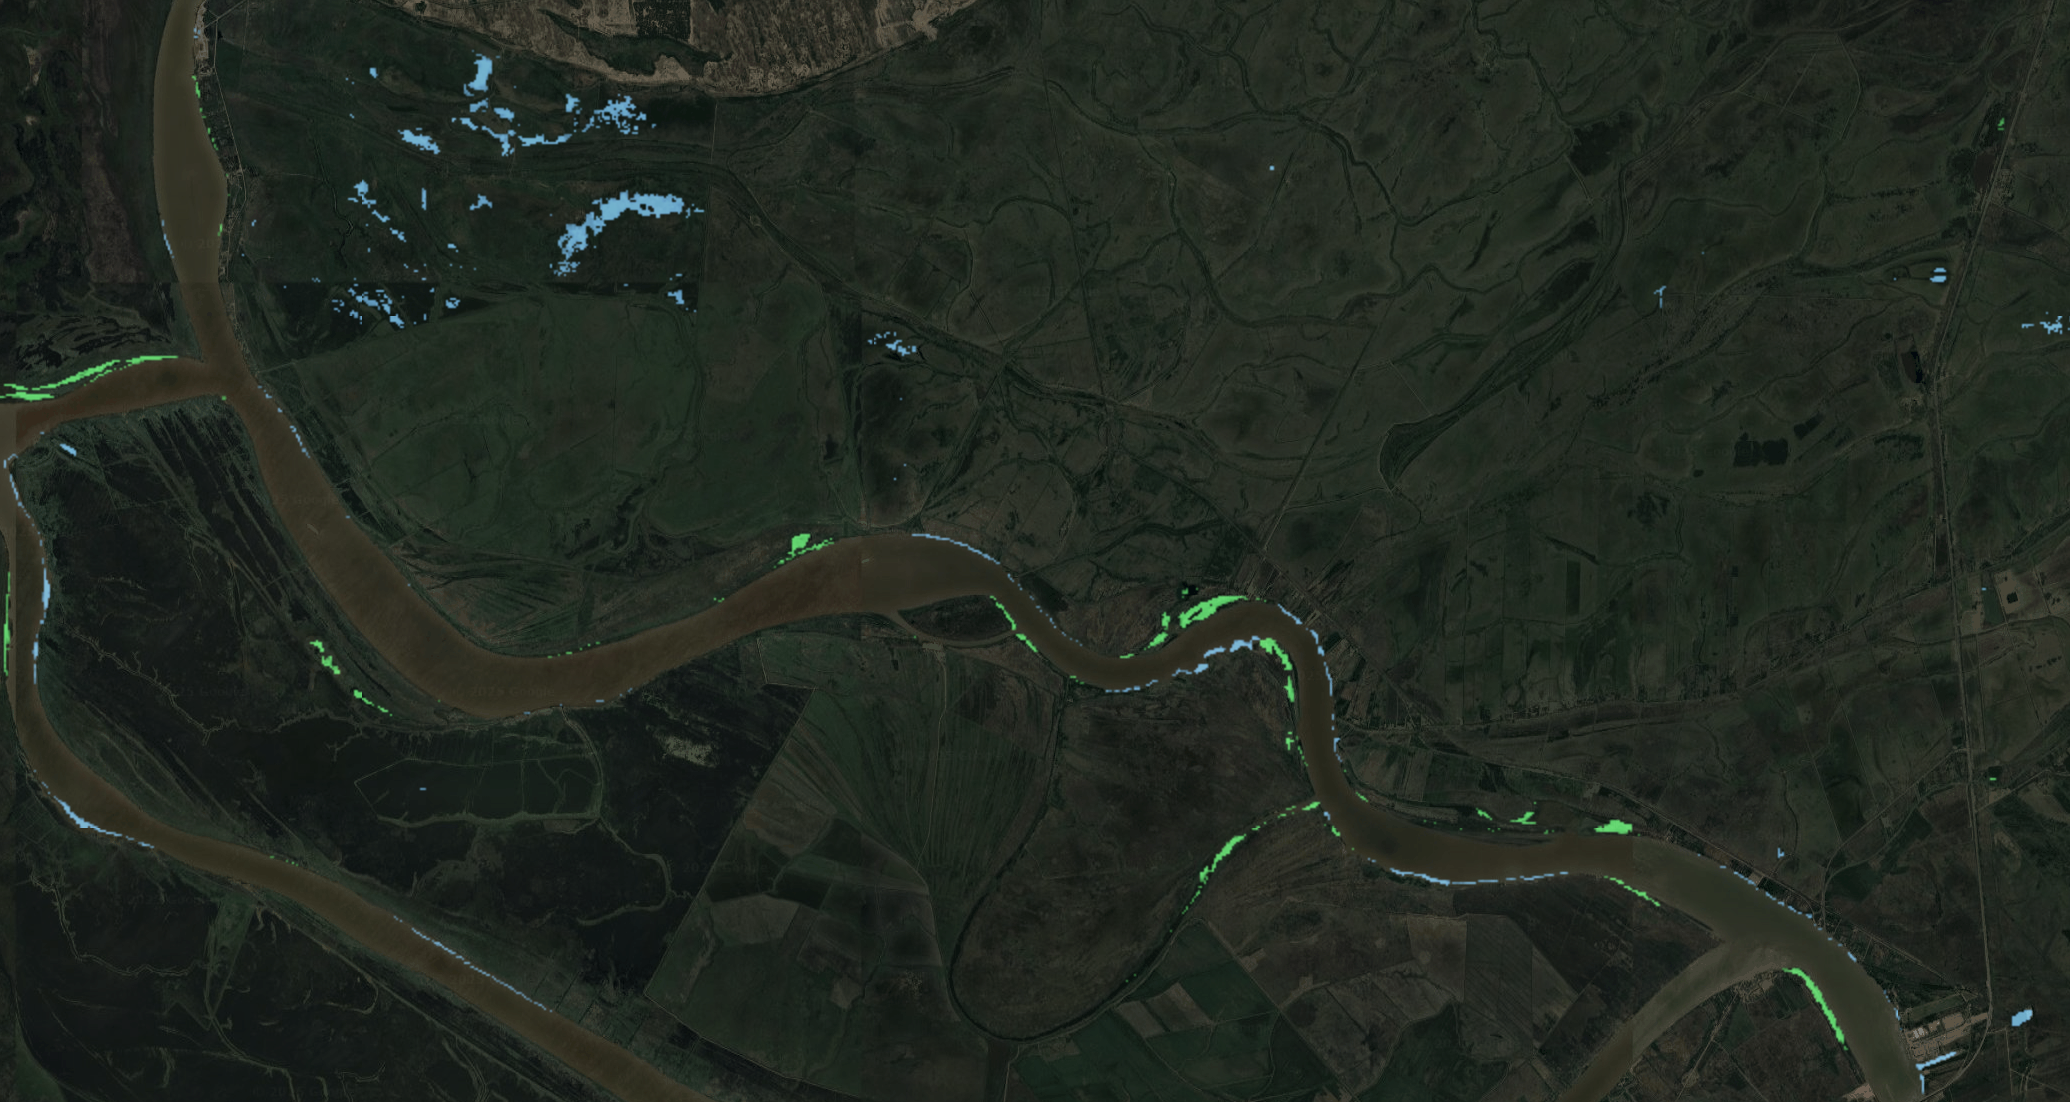
\includegraphics[width=\linewidth, height=5cm]{figures/ch8/critical_location_google.png}
        \caption{Critical location Aqua Monitor}
        \label{fig:critical_location_google}
    \end{subfigure}
    \hfill
    \begin{subfigure}[b]{0.45\textwidth}
        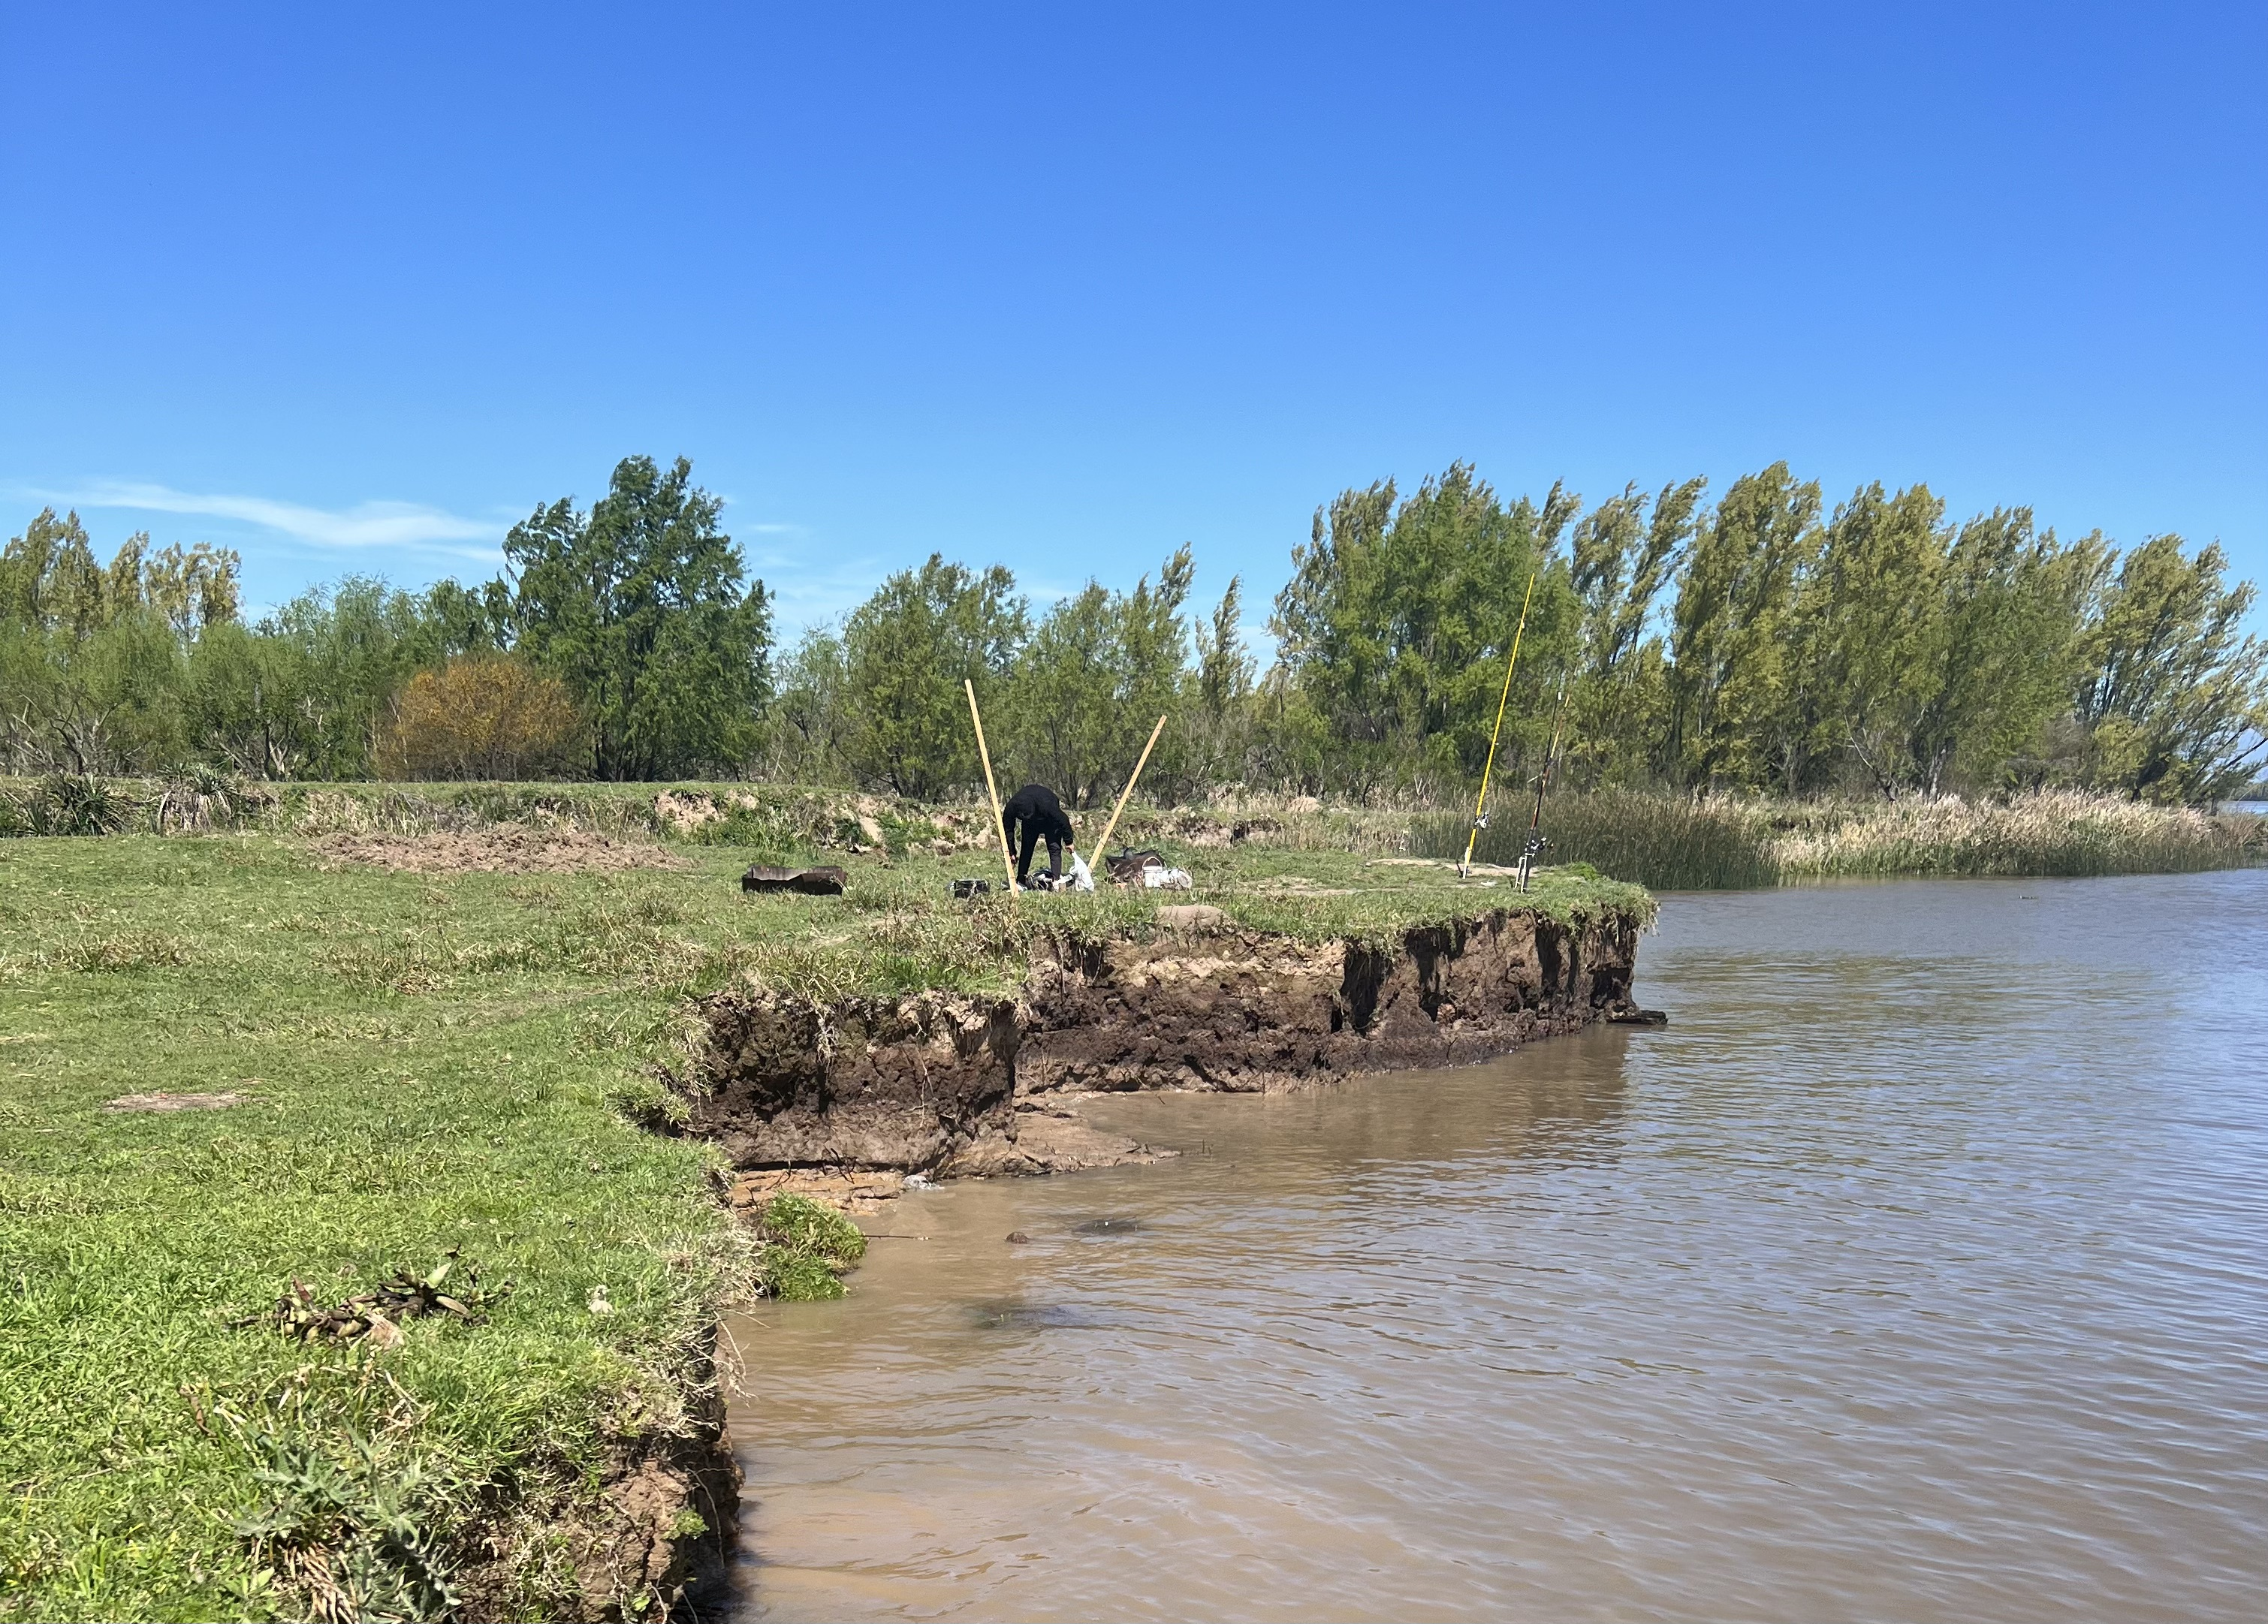
\includegraphics[width=\linewidth, height=5cm]{figures/ch8/critical_location.jpeg}
        \caption{Verification critical point field trip}
        \label{fig:critical_location_fieldtrip}
    \end{subfigure}
    \caption{Critical location}
    \label{fig:critical_location}
\end{figure}


\subsubsection{Problem description}

For the design of sheet pile wall in this section, the cantilever sheet pile wall will be used. As briefly touched on in Section \ref{section:sheet_pile_wall} the cantilever sheet pile is used for retaining heights up to 5 meters and is getting the support from the ground layers. In Figure \ref{fig:problem_description_sheetpiles}, an sketch of the situation is given. The height which need to be retained in indicated with Z. The embedment depth of the cantilever sheet pile which will need to be determined iterative, is noted as t. In this sketch the ground water table is indicated by the dashed line and abbreviation GWT. The water level of the river is indicated as WL and is in this sketch indicated by WL, which is on the same level as the GWT. 

\begin{figure}[H]
    \centering
    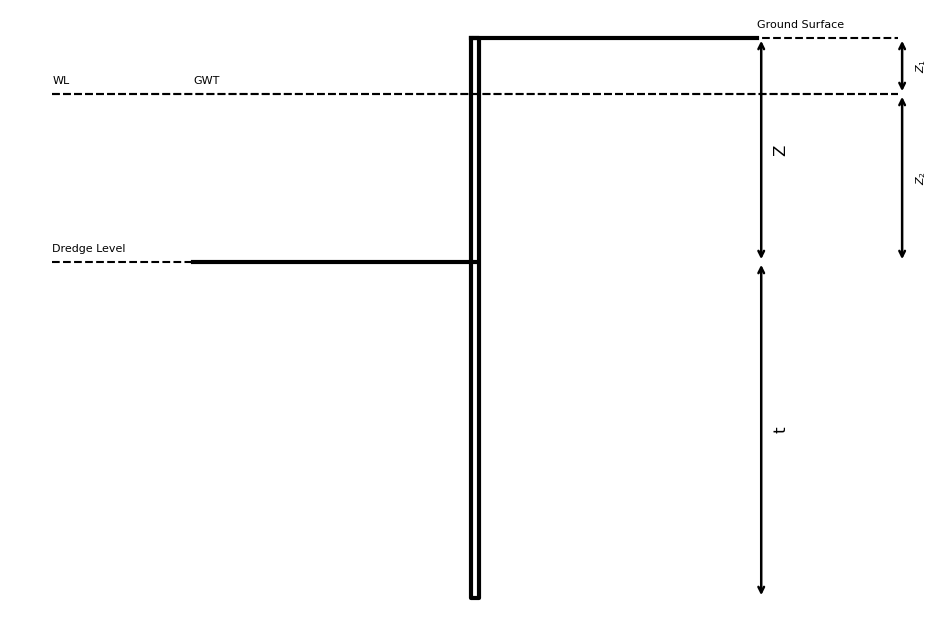
\includegraphics[width=0.70\linewidth]{figures/ch8/sketch_profile.png}
    \caption{Problem desciption sheet pile wall}
    \label{fig:problem_description_sheetpiles}
\end{figure}

\subsubsection{Method}

Hier bespreken welke desgin methode we gaan gebruiken. Active en Passive kant van de sheet pile bepalen. Kracht horizontal en momenten som aan nul gelijk stellen om daarmee te bepalen wat de D van de sheet pile moet zijn. Hier een factor overheen gooien. 

\subsubsection{Plan}

Hier komt de procedure te staan hoe het design tot stand zal gaan komen en welke stappen gemaakt zullen worden. Uitleggen dat het een iteratief process is om de D te vinden doormiddel van de krachten en momentensom. De momentensom moet 0 zijn onderaan en hiermee kan dan de D bepaald worden. \textbf{}

\subsubsection{Safety concept}

Structural requirements

\subsubsection{Soil parameters and profile}
To be able to design the sheetpile, the soil layers along with their geotechnical parameters should be known. In paragraph \ref{par:geology}, the geological background for the area of interest was given and this serves as the basis for deriving soil layers and parameters. The borehole in figure \ref{fig:borehole} is deemed the most relevant source. The borehole shows a top layer with fine/medium sands. Below, clay/clayey sand can be found, and the bottom layer consists of medium sand. This is in accordance with the geological profile that was provided before in figure \ref{fig:geolprofile}, which describes a transition from near-surface beach ridges, dunes, beach plains, and delta subaerial facies to deeper open estuaries and marine deposists. The top deposits help declare the presence of sandy deposits at the top of the borehole and the layers of clay/clayey sand below correspond to estuarine deposits. Finally, old marine/fluvial deposits were likely compacted and lead to the layer of medium sand found at the bottom of the borehole.

Because of the resemblance between the local borehole and the geological profile given before, the layering as shown in figure \ref{fig:borehole} is deemed representative for the whole study area. Based on this layering the relevant parameters can be derived, the result is shown in table \ref{tab:soil_layers}.

\begin{table}[H]
    \centering
    \begin{tabular}{|c|c|c|c|c|c|c|c|}
        \hline
        Start layer (m) & End layer (m) & Soil type & \makecell{ $\gamma_d$ \\ (kN/m$^3$) } & \makecell{ $\gamma_{sat}$ \\ (kN/m$^3$) } & \makecell{ $\varphi'$ \\ ($^\circ$) } & \makecell{ $c'$ \\ (kPa) } & \makecell{ $c_u$ \\ (kPa) } \\
        \hline
        0 & 2 & Fill (Topsoil/Agricultural) & 12 & 12 & 15 & 2.5 & 20 \\
        2 & 7 & Fine/medium sand & 17 & 19 & 30 & 0 & - \\
        7 & 10 & Clay & 14 & 14 & 17.5 & 0 & 25 \\
        10 & 15 & Clayey sand & 18 & 20 & 25 & 0 & - \\
        15 & 16 & Clay & 14 & 14 & 17.5 & 0 & 25 \\
        16 & 17.5 & Clayey sand & 18 & 20 & 25 & 0 & - \\
        17.5 & 32 & Medium sand & 18 & 20 & 32.5 & 0 & - \\
        \hline
    \end{tabular}
    \caption{Soil stratigraphy and geotechnical properties.}
    \label{tab:soil_layers}
\end{table}

The parameters in table \ref{tab:soil_layers} were derived from the Eurocode \autocite{stichtingkoninklijknederlandsnormalisatieinstituutNederlandseNormNEN2025}. Because of limited knowledge on soil characteristics, conservative estimates were made based on this code. In the borehole, no explicit information is given on the top fill layer. Therefore, conservative parameters were assumed based on typical values for organic topsoil.



Hier komt te staan wat de lengte en diepte van de sheet piles zullen worden. En welk profiel gebruikt zal worden voor de sheet piles. Ook de bepalende combinatie van rekenwaarde laten zien in een tabel.

\subsubsection{Loads}

Hier komt een beschrijving van de verschillende krachten die op de damwand komen te staan. Denk hierbij aan de earth pressure, water pressure en de golf energie force.

\subsubsection{Effective Stress}

Uitleg over hoe de effective stress berekend wordt met een afbeelding van de passive en active side en een tabel met de belangrijkste waarden. Uitleg dat alles onder de dredging line een waarden zal komen die uit een onbekende D zal bestaan.

\subsubsection{Hydrostatic Water Pressure}

Uitleg over hoe de hydrostatic water pressure berekend wordt met een afbeelding van de passive en active side en een tabel met de belangrijkste waarden. Uitleg dat alles onder de dredging line een waarden zal komen die uit een onbekende D zal bestaan.


\subsubsection{Earth Pressure}

Uitleg over hoe de active en passive earth pressure berekend wordt met een afbeelding en een tabel met de belangrijkste waarden. Uitleg dat alles onder de dredging line een waarden zal komen die uit een onbekende D zal bestaan. 

\subsubsection{Balance of Forces}

Vanuit de active en passive earth pressure de krachten kunnen bepalen doormiddel van vermenigvuldiging met de hoogte van de laag. Alle krachten laten zien in een tabel en ook een afbeelding van de krachten per driehoek en vierkant. Dit in de tabel mooi laten zien. Ook de balanssom van krachten beschrijven.

\subsubsection{Balance of Moments}

De momentensom om het laagste punt van de sheet pile gelijkstellen aan 0. Dit laten zien in een afbeelding en de uiteindelijke vergelijking die bestaat ui waardes en een onbekende D. Hieruit de wortel en d bepalen die de sheet pile zal moeten hebben. Ook een plaatje van de momenten lijn over de gehele damwand laten zien.

\subsection{Structural Verification}

\subsubsection{ULS and SLS}

\subsubsection{Normal Force}

\subsubsection{Moments}

\subsubsection{Deflection}

\subsection{Conclusion}

\section{Nature-based Solutions for dry sand mining}
Meer overheidsingrijpen nodig? Zie interview burgemeester: The judiciary forced the government to get involved: do controls, plan and regulate. Now there’s
a limit to extract, approx. 2 – 3 m. Before, there wasn’t.
En sed de arena report, overheid niet proactief genoeg

%https://www.unep.org/resources/report/sand-and-sustainability-10-strategic-recommendations-avert-crisis
%https://aapepyg.com/2022/11/23/fracking_entre_rios/#_edn4

While significant strides are taken to implement
nature-based solutions (NbS) against climate change
challenges, it is important to note that NbS requires large
volume of sand. Additionally, NbS may take time to have
the desired effect. Thus in some cases, grey structures
(i.e., concrete) may be necessary in the mean time to
address challenges in the short- to medium-term. In the
context of extreme heat and its impacts on cities, NbS
will also be instrumental to promote building designs and
materials that require neither concrete infrastructure nor
sand (UNEP 2021b). Climate change induced pressures,
such as temperature stress and precipitation, will also
speed up the degradation of existing infrastructure and
the need for upgrading or replacement
https://www.unep.org/resources/report/sand-and-sustainability-10-strategic-recommendations-avert-crisis

Op basis van uitgebreid, door deskundigen beoordeeld bewijsmateriaal concludeerde het Compendium van wetenschappelijke, medische en media-bevindingen die de risico's en schade van fracking aantonen, dat het niet mogelijk is om de techniek van de winning van onconventionele koolwaterstoffen 17Sed de Arena 2023 I Valeria Foglia en de daarmee samenhangende winningsactiviteiten niet mogelijk is zonder dat dit een bedreiging vormt voor de menselijke gezondheid, de lucht, het water, de economische vitaliteit op lange termijn, de biodiversiteit en de seismische en klimatologische stabiliteit. SED DE ARENA

This section seeks to propose and evaluate Nature-Based Solutions (NBS) that can effectively address the environmental and socio-economic consequences of dry sand mining. The analysis focuses on developing strategies that harness natural processes to restore degraded ecosystems, enhance landscape resilience, and promote sustainable resource management. In order to provide a comprehensive understanding, the potential advantages and limitations of each proposed NBS will be critically examined. Furthermore, this section will delineate the intended implementation framework, outlining the methodological approach and practical steps required to translate these solutions into effective, context-specific interventions.

\subsection{Floodplains}

Floodplains are low-lying areas around rivers that naturally flood during periods of high water discharge. When managed and restored appropriately, these zones play a crucial role in maintaining riverine ecosystem functions and mitigating the adverse impacts of human activities such as sand mining and land degradation.

In the context of dry sand mining, floodplains could be a Nature-Based Solution to counteract the degradation of terrestrial and hydrological systems resulting from excessive sand extraction. Dry sand mining frequently occurs in former floodplain areas or adjacent uplands, where the removal of surface materials disrupts soil structure, alters drainage patterns, and reduces the area’s natural capacity to retain water. Restoring and reactivating floodplains in such landscapes helps to re-establish the natural hydrological connectivity between surface and subsurface systems. This process promotes groundwater recharge, initiate soil sedimentation and mitigates erosion caused by wind and surface runoff. Moreover, re-vegetated floodplains provide new habitats for native species, contributing to the overall ecological recovery of mined areas. As such, floodplain restoration in dry sand mining zones supports landscape resilience, reduces the long-term environmental footprint of extraction activities, and facilitates a more sustainable post-mining land use.

Restored floodplains offer significant opportunities for local community engagement, livelihood diversification, and socio-economic development. Once stabilized and revegetated, these areas can be utilized for sustainable land uses such as flood-resilient agriculture, agroforestry, and controlled grazing, which maintain ecological functions while providing income for local populations. Additionally, floodplains can serve as sites for eco-tourism, recreation, and environmental education, fostering a stronger connection between communities and their natural surroundings. The enhancement of biodiversity and landscape aesthetics further increases the cultural and recreational value of these areas. Moreover, the restored floodplain’s role in improving water retention and soil fertility can directly support local food and water security, especially in regions affected by the environmental degradation of dry sand mining. Through community-based stewardship, floodplain restoration can therefore become a catalyst for sustainable rural development and long-term environmental resilience.

\subsubsection{Implementation in Ibicuy area}

\subsection{Vegetated buffer zones}
Vegetated buffer zones are strips of land planted with dense vegetation, such as grasses, shrubs, and trees, established between areas of active land use (dry mining sites) and surrounding environments such as settlements, agricultural fields and nature. In the context of dry sand mining, these buffers function as a natural barrier that mitigates the spread of dust, noise, and pollutants generated by extraction activities.

From an ecological perspective, vegetated buffer zones play a vital role in stabilizing soil, reducing wind speed, and capturing airborne particles, thereby improving local air quality and minimizing off-site impacts. The root systems of the plants anchor the sandy substrate, preventing erosion and surface runoff, while the vegetation canopy traps dust and enhances microclimatic conditions by increasing humidity and reducing temperature fluctuations.

In addition to their environmental benefits, buffer zones contribute to biodiversity enhancement by creating transitional habitats that support a variety of species and small fauna. They also serve as visual and acoustic screens, reducing noise and improving the aesthetic quality of the landscape. When designed with native and drought-tolerant species, vegetated buffers require minimal maintenance and can thrive in the disturbed conditions typical of mining landscapes.

Moreover, the establishment of buffer zones can provide socio-economic advantages for local communities through community-based planting initiatives. Overall, vegetated buffer zones represent a cost-effective and multifunctional Nature-Based Solution that simultaneously addresses environmental degradation, air quality concerns, and landscape restoration in areas affected by dry sand mining.
